\chapter{Introduction}
\label{chap:Introduction}

%The outcome of a builds tests and build steps are examples of data that is produced.
In recent years, software companies have started to generate much more data about their development processes as a result of the wide adoption of continuous integration. Fowler \cite{FowlerCI} defines continuous integration (CI) as a software practice where developers in a team integrate work frequently, typically once a day or more \cite{FowlerCI}. Each integration is then verified by an automated build that runs tests, checks for code standard violations etc.\ \cite{FowlerCI}. According to Duval et.\ al \cite{CIbook}, the proposed benefits of using CI include an increased project visibility where problems like failing builds can be noticed instantly. Therefore, data generated through the use of CI is crucial to the success of the practice, since CI stresses the need for transparency, information sharing and information visualization \cite{FowlerCI, CIbook}. Collecting this data also opens up companies to analyze trends about their development processes in the long term \cite{CIbook, bigDataMane}. However, Schram and Anderson \cite{MySQLToNoSQL} state that having software systems that generate large amounts of data on a daily basis is not without consequence and likely introduces challenges. These include having the appropriate technical infrastructure and software in place to deal with data growth and also supporting different use cases for operating on collected data.

The company Ericsson recently began adoption of continuous integration. At the company, there are two high level use cases for data collected from the continuous integration process. The first is to visualize newly created data, in real time, to developers. The second is to perform analytics, making use of historical data. This use case is of interest for the management staff as a means to quantify the effectiveness of the development process, to see if for example the proportion of successful builds increase over time.


%This is an important part of lean \cite{lean}.
 %These use cases in combination with the monotonic growth of the total amount of collected data from the continuous integration process leads to a number of technical considerations when developing and evolving CIMS.

Since the adoption of continuous integration at Ericsson, several software systems in support of this process have been put into use, including a web application developed internally called CIMS (Continuous Integration Management System). It has several instances, one for each of the larger software products being developed, and its main purpose is to address the first high level use case, namely to visualize data for developers. However, it is currently also used for the second use case.

Recently it has been observed that the amount of builds registered into CIMS is increasing. At the same time the amount of test cases for each build is also increasing. The technology stack of CIMS was originally not made to scale with this rate of monotonic growth which in turn has introduced problems that impact performance, maintainability, changeability and other factors.

The influx of data for one of the larger developed software products are shown in figure~\ref{fig:jeTrend}. The trend is increasing, with different factors involved in describing why it looks like it does. As the situation is today, the data growth this trend describes has caused a variety of problems with the current infrastructure supporting the continuous integration process.

%This figure clearly shows the trend in the data inflow of CIMS.
\begin{figure}[h!]
\centering
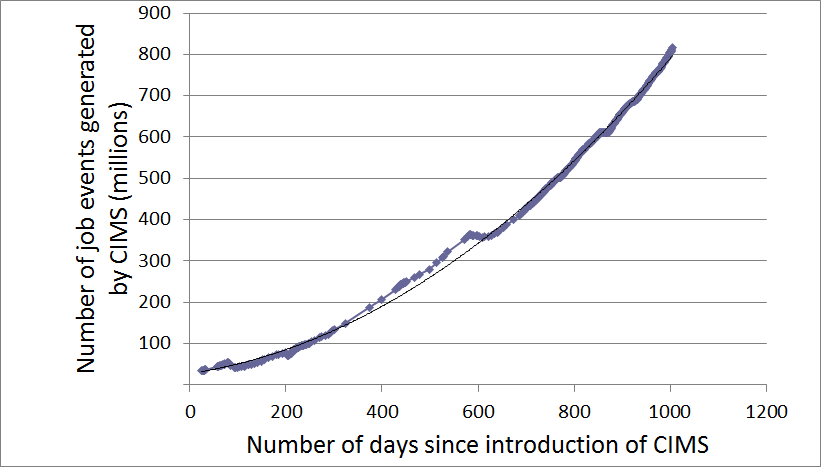
\includegraphics[scale=0.65]{figure/jeTrend.png}
\caption{Diagram showing the data growth for one instance of CIMS.}
\label{fig:jeTrend}
\end{figure}

One of these problems with the current implementation of CIMS stems from the need to evolve the system, specifically its data model and schemas. Currently, all system data is stored in a single relational database. For evolution to take place, all data must be migrated to match new versions of the system. At current rates of stored data, these migrations can take as much as a week's time to complete. Due to the long running migrations, the evolution of CIMS is impaired. This has halted efforts to improve the continuous integration process, thus reducing Ericsson's ability to respond to market changes.

\section{Problem description}
The context for this thesis is the intersection of continuous integration systems and data management. The focus is on the management of historical data and problems related to monotonic data growth. As such, we have broken down the research problem into two parts; the first part is to investigate different solutions to manage historical data that grows monotonically. The second part is to justify the value of having a solution by understanding how historical data in continuous integration systems can be used and what value it brings to the organization that possess the data. 

Both these problems were addressed using a design research approach. This approach is described in detail in the sections \ref{purpose}, \ref{method} and \ref{objectives} where we also present the research purpose and research questions.

\section{Research Purpose}
\label{purpose}
The purpose of this study is to identify and evaluate solutions for management of historical data in a continuous integration system, more specifically, to evaluate the suitability of polyglot persistence (see section~\ref{sec:pp}) in that context. Based on the problem description and the research purpose, we ask the following research questions:

RQ1: How can historical data in continuous integration systems be managed in the long term? \\
RQ2: What value can a solution to management of historical data in continuous integration systems bring to an organization?
%RQ2: Does the value gained from solving the problem of monotonic growth in continuous integration systems outweigh the identified costs related to implementing a solution for the problem? \\

\section{Research Method}
\label{method}
This thesis will be conducted using design research methods based on knowledge from \cite{DS, Peffers, DesignEval}. Design research is performed by building and evaluating artifacts that are designed with the purpose of addressing a specified business need or problem \cite{DS}. 

Peffers et al.\ \cite{Peffers} describe an overall process for conducting design research which for the purposes of this thesis has been implemented as in figure~\ref{fig:peffer}. As can be noted in this figure, one important aspect of design research is its focus on iterative processes, where evaluation should inform reformulation of solution objectives and also give feedback to upcoming iterations of design and development. This part of the process will be implemented by performing several iterations of design/development and demonstration/evaluation. If necessary, solution objectives can be changed as an increased understanding of the problem is gained. 

According to \cite{Peffers}, there are several possible entry points for a design research study. In our case the entry point is an objective-centered solution, since the need for the study originated from an industrial problem that could be addressed by constructing an artifact.
\begin{figure}[h!]
\centering
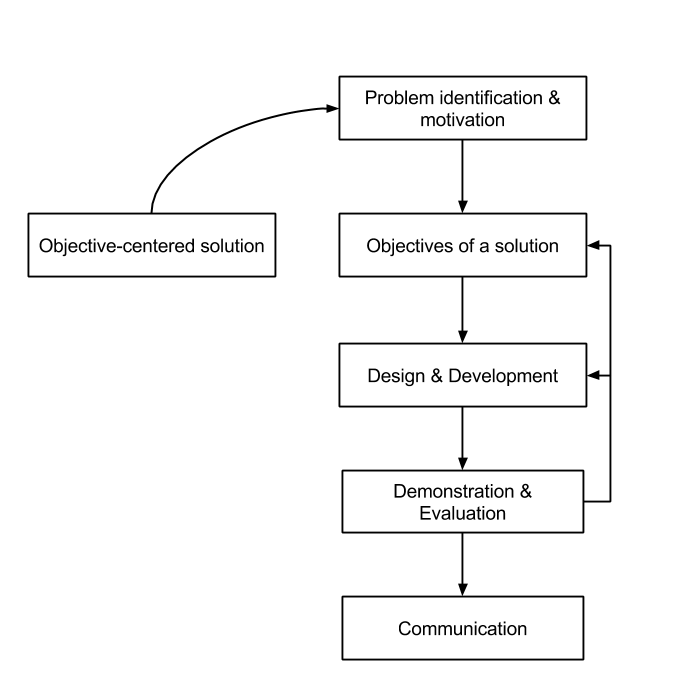
\includegraphics[width=0.7\pdfpagewidth]{figure/Peffer.png}
\caption{The design research process as described in \cite{Peffers}.}
\label{fig:peffer}
\end{figure}

In this thesis, our implementation of the process described by Peffers et al.\ \cite{Peffers} laid out the overall framework used to design the study. First, we studied and defined the problem in more detail in collaboration with the CIMS development team. After this, we proceeded with the formulation of solution objectives which set the scope for this thesis. During this process, an overview of related work was written.

With solution objectives in place, work began on the two bigger phases, namely design/development and evaluation. In a given iteration of design/development, an artifact in the form of a prototype was either built from scratch or further developed.

For the evaluation process, options given by \cite{DesignEval} were used to define properties of the artifact, its purpose and actual approaches used for evaluation. The choices made are shown in figure~\ref{fig:matrix}.

Further explanations of some of these choices are warranted; the goal of the evaluation is to gather knowledge about the problem and its domain so as to put upcoming decisions made at Ericsson on a rational basis. As such, evaluation goes in line with the knowledge function described in \cite{DesignEval}. 

A prototype solution was requested by stakeholders at Ericsson which is why the choice was made to evaluate using this method. Since we evaluate a prototype it is the artifact itself that is evaluated as opposed to the construction of the artifact.

Given that the thesis was conducted in collaboration with Ericsson, the artifact was evaluated in an organizational context and as such against the real world. Finally, we chose to do evaluation after the construction (ex post) of the artifact.

\begin{figure}[h!]
\centering
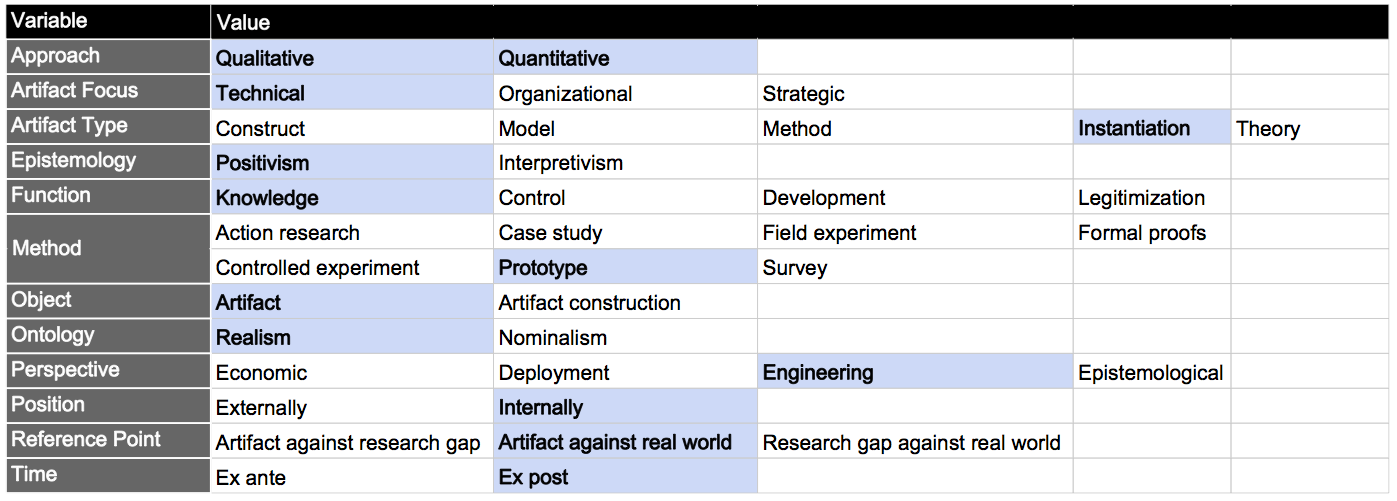
\includegraphics[width=0.7\pdfpagewidth]{figure/eval.png}
\caption{Evaluation matrix. Choices made are marked in bold and colored.}
\label{fig:matrix}
\end{figure}


\section{Solution objectives}
\label{objectives}
In adherence with the design research process, a set of objectives that define a successful solution has been defined in collaboration with the CIMS development team. The main objective is to develop an archive system that physically separates stale data from live data in order to further support the evolution of CIMS.

While stale data is not accessed often, it is still useful for analytics purposes and to respond to trouble reports from customers running older versions of Ericsson products. Therefore a secondary objective is to retain as much functionality as possible in terms of queries on the archived portion of the data. The specific queries that the archive should support have been defined through discussion with the CIMS development team and the metrics team.

For the combination of CIMS and the archive system to be future proof it must also be able to scale better with overall data size than CIMS currently does. This ensures that the problem is simply not pushed further into the future but rather solved in its entirety.

In summary, 3 main objectives have been identified. They are as follows;
\begin{enumerate}
\item Develop an archive solution that physically separates live from stale data.
\item Retain a set of important queries on archived data.
\item Introduce long term scalability.
\end{enumerate}

%3. Handle structural variation on incoming data to the archive.\\
%Physical separation of live and stale data means that the storage solution for archived data must be flexible enough to handle structure variation on incoming data. If it does not then the problem of long running migrations is not solved but rather moved to the data store of the archive. 

\section{Report structure}
This report is structured in the following way; In chapter~\ref{chap:background} the background and related work is described. Chapter~\ref{chap:domain} describes the domain of CIMS and the business context in more detail. In chapter~\ref{chap:design} a description is given of how the artifact addressing the identified problem was designed and implemented.
This is followed in chapter~\ref{chap:eval} by a description of how the artifact was evaluated. Results and discussion of this evaluation are given in chapter~\ref{chap:results}. The report is then wrapped up in chapter~\ref{chap:conclusion} with conclusions.

%Relational databases have been the standard for data storage in a wide range of domains and applications since the 1970s \cite{Codd}. Many attempts have been made to replace them but none have yet to succeeded in a meaningful way \cite{NoSQLDistilled}.

%The wide adoption and success of the concept Continuous Integration has led to an  
%Monotonic Increasing/Rel DB -> Historical Data -> Continuous Integration -> Ericsson

%\section{Problem identification}
%
%Organizations often find themselves in a situation where the requirements of a software system have emergent properties that were not planned for. In this thesis, the emergent problem that has been identified is that of unplanned and large data growth. To manage this problem, one of the first responses is often to physically separate stale data from live data \cite{Mullins}.
%
%In addition to increased complexity, Curino et al.\ \cite{Moon09} state that the relational model alone is too restrictive for storing and querying evolving historical data. However, polyglot persistence has shown promise in this area \cite{Moon05, Moon09, MoonPHD}. In \cite{Moon09}, a solution is described where XML is used to store historical data along with mappings between schema versions. The solution is reported to provide a unified query interface on all different schema versions of the historical data. However, XML databases are noted to scale poorly \cite{Moon09} and XML as a data format for semi-structured data is considered less than ideal \cite{JSONData}. As a comparison, the JSON format is simpler \cite{JSONData} and more widely adopted by newer NoSQL databases \cite{Catell}.
%
%Given the mentioned issues regarding XML databases, other non relational storage options should be evaluated for storing evolving historical data. The emergence of the NoSQL movement has led to comparative studies \cite{Catell, NoSQLSurvey} which are relevant for this evaluation. This research has later been extended with knowledge on how to use different NoSQL databases in the same system \cite{NoSQLDistilled} and how to use both SQL and NoSQL databases in the same system \cite{MySQLToNoSQL}. However, the research field of databases lack studies investigating the practical suitability of polyglot persistence solutions with evolving historical data.
%

%\begin{figure}[h!]
%\centering
%\includegraphics[width=0.45\linewidth, trim=3cm 11cm 3cm 11cm]{figure/X.pdf}
%\includegraphics[width=0.45\linewidth, trim=3cm 11cm 3cm 11cm]{figure/Y.pdf}
%\caption{Surface and contour plots showing the two dimensional function\\ $z(x,y)=\sin(x+y)\cos(2x), x\in [0,2], y\in [0,1]$.}
%\end{figure}
%
%\section{Equation}
%\begin{equation}
%f(t)=\left\{ \begin{array}{ll}
%1,~~~~ & t< 1 \\
%t^2 & t\geq 1
%\end{array}\right.
%\end{equation}
%
%\section{Table}
%\begin{table}[h!]
%\centering
%\caption{Values of $f(t)$ for $t=0,1,\dots 5$.}
%\begin{tabular}{l|llllll} \hline\hline
%$t$ & 0 & 1 & 2 & 3 & 4 & 5 \\ \hline
%$f(t)$ & 1 & 1 & 4 & 9 & 16 & 25 \\ \hline\hline
%\end{tabular}
%\end{table}
%
%\section{Chemical structure}
%\begin{center}
%\chemfig{X*5(-E-T-A-L-)}
%\end{center}
%
%
%\section{List}
%\begin{enumerate}
%  \item The first item
%  \begin{enumerate}
%    \item Nested item 1
%    \item Nested item 2
%  \end{enumerate}
%  \item The second item
%  \item The third item 
%  \item \dots
%\end{enumerate}
%
%\section{Source code listing}
%%\lstset{language=Matlab}
%\begin{lstlisting}[frame=single]
%% Generate x- and y-nodes
%x=linspace(0,1); y=linspace(0,1);
%
%% Calculate z=f(x,y)
%for i=1:length(x)
% for j=1:length(y)
%  z(i,j)=x(i)+2*y(j);
% end
%end
%\end{lstlisting}


%The relational database in use today is not ideal for storing the large amount of historical data that is considered to be stale. As stated earlier, this stale data is still valuable for analytical purposes. Therefore, just deleting stale data in order to enable evolution of CIMS is not a viable option.

%However, a large portion of the data is considered stale as it is not accessed on a daily basis.

%Varför tas inte bara datan bort? Jo för man vill ju kunna göra Buisness analysis blabla på den.

%In this thesis, a solution to archiving of historical data was developed and evaluated using a design research approach. The practical suitability of a polyglot persistence solution using NoSQL as an alternative was explored in depth. The thesis was conducted at Ericsson as a response to an identified problem with an existing system that aggregates and visualizes data from software build systems and continuous integration workflows.

%Benefits: \\
%- Offload live database. By keeping the size of the live database manageable the need for scaling up the hardware it runs on is lessened. It will also be much more performant. The possibility to continuously evolve and deploy CIMS instances is won back. Finally it will be reduced to fulfilling one main task; serving CIMS with data.
%- Hardware cost reduction.\\
%- Enable continuous integration and deployment of CIMS.\\
%- Increased performance of live database.\\
%- Make analytics possible.\\
%- Full history kept.\\

%Drawbacks:\\
%- Cost of implementing solution.\\
%- Train staff in new technology or hire new staff with the skills needed.\\
%- Increased complexity of CIMS and its related systems.\\
%- New code to maintain\\

%A consequence of moving towards continuous integration is certainly that an organization will start to collect much more data about its software development process. The value of this data is defined by how it is used. If it is never used for anything in particular then it should just be purged on a regular basis to keep databases at a manageable size. This is however not likely to be the case. As such, a number of benefits can be observed by solving the data growth problem. Drawbacks also exist.
